% Source: graduate-coursework/Research/Intro_to_Agents/handouts/Part4_Planning_Workflow.tex

\documentclass[border=4pt]{standalone}
\usepackage{graphicx}
\usepackage{tikz}
\usepackage{xcolor}
\usetikzlibrary{shapes.geometric, arrows.meta, positioning, calc, fit, backgrounds}

\definecolor{UofSCGarnet}{HTML}{73000A}
\definecolor{UofSCBlack}{HTML}{000000}
\definecolor{UofSCWhite}{HTML}{FFFFFF}
\definecolor{UofSCAtlantic}{HTML}{466A9F}
\definecolor{UofSCCongaree}{HTML}{1F414D}
\definecolor{UofSCHorseshoe}{HTML}{65780B}
\definecolor{UofSCRose}{HTML}{CC2E40}
\definecolor{UofSCDarkGarnet}{HTML}{570008}
\definecolor{UofSC90Black}{HTML}{363636}
\definecolor{UofSC70Black}{HTML}{5C5C5C}
\definecolor{UofSC50Black}{HTML}{A2A2A2}

\tikzset{
    box/.style={
        draw=UofSCBlack,
        fill=#1,
        minimum width=2.5cm,
        minimum height=0.8cm,
        text=UofSCWhite,
        font=\small\bfseries,
        align=center,
        inner sep=4pt
    },
    box/.default=UofSCGarnet,
    lightbox/.style={
        draw=UofSCBlack,
        fill=UofSCWhite,
        minimum width=2.5cm,
        minimum height=0.8cm,
        text=UofSCBlack,
        font=\small,
        align=center,
        inner sep=4pt
    },
    arrow/.style={
        ->,
        >=Stealth,
        thick,
        UofSCBlack
    },
    bigarrow/.style={
        ->,
        >=Stealth,
        line width=1.5pt,
        UofSCGarnet
    },
    phase/.style={
        draw=UofSCBlack,
        fill=#1,
        minimum width=3cm,
        minimum height=1cm,
        text=UofSCWhite,
        font=\bfseries,
        align=center
    },
    phase/.default=UofSCGarnet,
    subphase/.style={
        draw=UofSC70Black,
        fill=UofSCWhite,
        minimum width=2.8cm,
        minimum height=0.6cm,
        text=UofSCBlack,
        font=\scriptsize,
        align=center
    },
    cyclebox/.style={
        draw=UofSCBlack,
        line width=1.5pt,
        fill=#1,
        minimum width=2cm,
        minimum height=1.2cm,
        text=UofSCWhite,
        font=\bfseries,
        align=center
    },
    cyclebox/.default=UofSCGarnet
}

\begin{document}
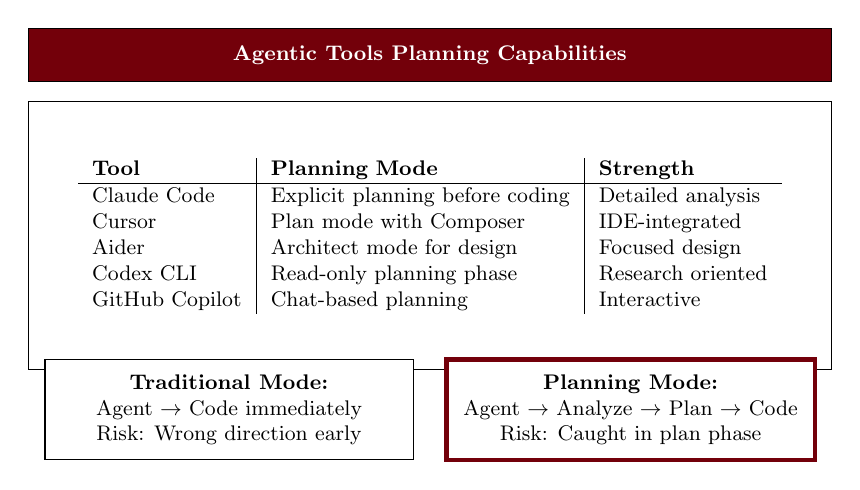
\begin{tikzpicture}[scale=0.85, transform shape]
        % Header
        \node[box=UofSCGarnet, minimum width=12cm] at (0,3) {Agentic Tools Planning Capabilities};

        % Table
        \node[lightbox, minimum width=12cm, minimum height=4cm, text width=11.5cm] at (0,0.3) {
            \begin{tabular}{l|l|l}
            \textbf{Tool} & \textbf{Planning Mode} & \textbf{Strength} \\
            \hline
            Claude Code & Explicit planning before coding & Detailed analysis \\
            Cursor & Plan mode with Composer & IDE-integrated \\
            Aider & Architect mode for design & Focused design \\
            Codex CLI & Read-only planning phase & Research oriented \\
            GitHub Copilot & Chat-based planning & Interactive \\
            \end{tabular}
        };

        % Bottom comparison
        \node[lightbox, minimum width=5.5cm, minimum height=1.5cm] at (-3,-2.3) {
            \textbf{Traditional Mode:}\\
            Agent $\rightarrow$ Code immediately\\
            Risk: Wrong direction early
        };
        \node[lightbox, minimum width=5.5cm, minimum height=1.5cm, draw=UofSCGarnet, line width=1.5pt] at (3,-2.3) {
            \textbf{Planning Mode:}\\
            Agent $\rightarrow$ Analyze $\rightarrow$ Plan $\rightarrow$ Code\\
            Risk: Caught in plan phase
        };
    \end{tikzpicture}
\end{document}
